\documentclass[docid=2017/18]{tcom_exam}
\begin{document}
\setcounter{section}{16}
\section{Exam 2017/18}
{
\renewcommand{\thesubsubsection}{\thesubsection\alph{subsubsection}}
\subsection{Group I}
\subsubsection{Item a}
\begin{alignat*}{2}
	&\varepsilon close(q_0&&)=\{q_0,q_1,q_2,q_3\}\\
	&\varepsilon close(q_1&&)=\{q_1,q_2,q_3\}\\
	&\varepsilon close(q_2&&)=\{q_2\}\\
	&\varepsilon close(q_3&&)=\{q_3\}\\
	&\varepsilon close(q_4&&)=\{q_3,q_4\}
\end{alignat*}
\subsubsection{Item b}
\begin{minipage}[c]{0.7\textwidth}
	\begin{center}
		\begin{tabular}{r | c c}
			$\delta_D$                            & $a$ & $b$ \\ \hline
			$            \emptyset              $ & $\emptyset$ & $\emptyset$ \\
			$         ^* \{            q_3,q_4\}$ & $\{q_3,q_4\}$ & $\emptyset$\\
			$         ^* \{        q_2,q_3,q_4\}$ & $\{q_3,q_4\}$ & $\{q_3,q_4\}$\\
			$\rightarrow \{q_0,q_1,q_2,q_3    \}$ & $\{q_0,q_1,q_2,q_3,q_4\}$ & $\{q_2,q_3,q_4\}$ \\
			$         ^* \{q_0,q_1,q_2,q_3,q_4\}$ & $\{q_0,q_1,q_2,q_3,q_4\}$ & $\{q_2,q_3,q_4\}$
		\end{tabular}
	\end{center}
\end{minipage}
\begin{minipage}[c]{0.29\textwidth}
	\begin{center}
		\begin{tabular}{r | c c}
			$\delta_D$      & $a$ & $b$ \\ \hline
			$    \emptyset$ & $\emptyset$ & $\emptyset$ \\
			$         ^* A$ & $A$ & $\emptyset$\\
			$         ^* B$ & $A$ & $A$\\
			$\rightarrow C$ & $D$ & $B$ \\
			$         ^* D$ & $D$ & $B$
		\end{tabular}
	\end{center}
\end{minipage}
\begin{center}
	\begin{tikzpicture}[->,>=stealth',node distance=2cm,initial text=$ $,]
		\node[state, initial						] (C) {$C$};
		\node[state, accepting, above right of=C	] (D) {$D$};
		\node[state, accepting, below right of=D	] (B) {$B$};
		\node[state, accepting, right of=B			] (A) {$A$};
		\node[state, right of=A						] (e) {$\emptyset$};

		\draw	(e)	edge[loop above	] node{$a,b$} (e)

				(A)	edge[loop above	] node{$a$} (A)
				(A)	edge[above		] node{$b$} (e)

				(B)	edge[above		] node{$a,b$} (A)

				(C)	edge[left		] node{$a$} (D)
				(C) edge[above		] node{$b$} (B)

				(D)	edge[loop above	] node{$a$} (D)
				(D)	edge[right		] node{$b$} (B)
				;
	\end{tikzpicture}
\end{center}
\subsubsection{Item c}
\begin{minipage}[c]{0.49\textwidth}
	\begin{center}
		\begin{tabular}{r || c | c | c | c | c}
						& $\emptyset$ & $^* A$ & $^* B$ & $C$ & $^* D$ \\ \hline \hline
			$\emptyset$ & \cellcolor{gray} & \cellcolor{gray}    & \cellcolor{gray}    & \cellcolor{gray}    & \cellcolor{gray}    \\ \hline
			$     ^* A$ & X           & \cellcolor{gray}    & \cellcolor{gray}    & \cellcolor{gray}    & \cellcolor{gray}    \\ \hline
			$     ^* B$ & X           &     &  \cellcolor{gray}   & \cellcolor{gray}    & \cellcolor{gray}    \\ \hline
			$        C$ &             & X   & X   & \cellcolor{gray}    & \cellcolor{gray}    \\ \hline
			$     ^* D$ & X           &     &     & X   & \cellcolor{gray}    
		\end{tabular}
	\end{center}
\end{minipage}
\begin{minipage}[c]{0.49\textwidth}
	\begin{center}
		\begin{tabular}{r || c | c | c | c | c}
						& $\emptyset$ & $^* A$ & $^* B$ & $C$ & $^* D$ \\ \hline \hline
			$\emptyset$ & \cellcolor{gray} & \cellcolor{gray}    & \cellcolor{gray}    & \cellcolor{gray}    & \cellcolor{gray}    \\ \hline
			$     ^* A$ & X           & \cellcolor{gray}    & \cellcolor{gray}    & \cellcolor{gray}    & \cellcolor{gray}    \\ \hline
			$     ^* B$ & X           & X   &  \cellcolor{gray}   & \cellcolor{gray}    & \cellcolor{gray}    \\ \hline
			$        C$ & X           & X   & X   & \cellcolor{gray}    & \cellcolor{gray}    \\ \hline
			$     ^* D$ & X           & X   & X   & X   & \cellcolor{gray}    
		\end{tabular}
	\end{center}
\end{minipage} \vspace*{1em} \\
All states are distinguishable, so the automaton is already minimized.
\pagebreak
\subsubsection{Item d}
\begin{minipage}[c]{0.33\textwidth}
	\begin{center}
		\begin{tikzpicture}[->,>=stealth',node distance=2cm,initial text=$ $,]
			\node[state, accepting, initial				] (1) {$1$};
			\node[state, accepting, above right of=1	] (2) {$2$};
			\node[state, accepting, below right of=1	] (3) {$3$};
			\node[state, below right of=2				] (4) {$4$};

			\draw	(1)	edge[left				] node{$a$} (2)
					(1)	edge[left				] node{$b$} (3)

					(2)	edge[right				] node{$a$} (4)
					(2)	edge[bend left=10,right	] node{$b$} (3)

					(3)	edge[bend left=10,left	] node{$a$} (2)
					(3)	edge[right				] node{$b$} (4)

					(4)	edge[loop above			] node{$a,b$} (4)
					;
		\end{tikzpicture}
	\end{center}
\end{minipage}
\begin{minipage}[c]{0.33\textwidth}
	\begin{center}
		\begin{tikzpicture}[->,>=stealth',node distance=2cm,initial text=$ $,]
			\node[state, accepting, initial				] (1) {$1$};
			\node[state, accepting, above right of=1	] (2) {$2$};
			\node[state, accepting, below right of=1	] (3) {$3$};
			\node[state, below right of=2				] (4) {$4$};

			\draw	(1)	edge[left				] node{$a$} (2)
					(1)	edge[left				] node{$b$} (3)

					(2)	edge[right				] node{$a$} (4)
					(2)	edge[bend left=10,right	] node{$b$} (3)

					(3)	edge[bend left=10,left	] node{$a$} (2)
					(3)	edge[right				] node{$b$} (4)

					(4)	edge[loop above			] node{$a+b$} (4)
					;
		\end{tikzpicture}
	\end{center}
\end{minipage}
\begin{minipage}[c]{0.33\textwidth}
	\begin{center}
		\begin{tikzpicture}[->,>=stealth',node distance=2cm,initial text=$ $,]
			\node[state, accepting, initial				] (1) {$1$};
			\node[state, accepting, above right of=1	] (2) {$2$};
			\node[state, accepting, below right of=2	] (3) {$3$};

			\draw	(1)	edge[left				] node{$a$} (2)
					(1)	edge[below				] node{$b$} (3)

					(2)	edge[bend left=10,right	] node{$b$} (3)

					(3)	edge[bend left=10,left	] node{$a$} (2)
					;
		\end{tikzpicture}
	\end{center}
\end{minipage}
\begin{center}
	\begin{tabular}{c | c | c}
		\begin{minipage}[c]{0.30\textwidth}
			\begin{center}
				\begin{tikzpicture}[->,>=stealth',node distance=2cm,initial text=$ $,]
					\node[state, accepting, initial	] (1) {$1$};
					\node[state, above right of=1	] (2) {$2$};
					\node[state, below right of=2	] (3) {$3$};

					\draw	(1)	edge[left				] node{$a$} (2)
							(1)	edge[below				] node{$b$} (3)

							(2)	edge[bend left=10,right	] node{$b$} (3)

							(3)	edge[bend left=10,left	] node{$a$} (2)
							;
				\end{tikzpicture} \vspace*{1em} \\
				\begin{tikzpicture}[->,>=stealth',node distance=2cm,initial text=$ $,]
					\node[state, accepting, initial	] (1) {$1$};
					\node[state, right of=1	] (3) {$3$};

					\draw	(1)	edge[below				] node{$b+ab$} (3)
							(3) edge[loop above			] node{$ab$} (3)
							;
				\end{tikzpicture} \vspace*{1em} \\
				\begin{tikzpicture}[->,>=stealth',node distance=2cm,initial text=$ $,]
					\node[state, accepting, initial	] (1) {$1$};
				\end{tikzpicture}
				\begin{equation*}
					\varepsilon
				\end{equation*}
			\end{center}
		\end{minipage}&
		\begin{minipage}[c]{0.30\textwidth}
			\begin{center}
				\begin{tikzpicture}[->,>=stealth',node distance=2cm,initial text=$ $,]
					\node[state, initial						] (1) {$1$};
					\node[state, accepting, above right of=1	] (2) {$2$};
					\node[state, below right of=2				] (3) {$3$};

					\draw	(1)	edge[left				] node{$a$} (2)
							(1)	edge[below				] node{$b$} (3)

							(2)	edge[bend left=10,right	] node{$b$} (3)

							(3)	edge[bend left=10,left	] node{$a$} (2)
							;
				\end{tikzpicture} \vspace*{1em} \\
				\begin{tikzpicture}[->,>=stealth',node distance=2cm,initial text=$ $,]
					\node[state, initial				] (1) {$1$};
					\node[state, accepting, right of=1	] (2) {$2$};

					\draw	(1)	edge[above				] node{$a+ba$} (2)

							(2) edge[loop above			] node{$ba$} (2)

							;
				\end{tikzpicture}
				\begin{equation*}
					(a+ba)(ba)^*
				\end{equation*}
			\end{center}
		\end{minipage} &
		\begin{minipage}[c]{0.30\textwidth}
			\begin{center}
				\begin{tikzpicture}[->,>=stealth',node distance=2cm,initial text=$ $,]
					\node[state, initial						] (1) {$1$};
					\node[state, above right of=1				] (2) {$2$};
					\node[state, accepting, below right of=2	] (3) {$3$};

					\draw	(1)	edge[left				] node{$a$} (2)
							(1)	edge[below				] node{$b$} (3)

							(2)	edge[bend left=10,right	] node{$b$} (3)

							(3)	edge[bend left=10,left	] node{$a$} (2)
							;
				\end{tikzpicture} \vspace*{1em} \\
				\begin{tikzpicture}[->,>=stealth',node distance=2cm,initial text=$ $,]
					\node[state, initial				] (1) {$1$};
					\node[state, accepting, right of=1	] (3) {$3$};

					\draw	(1)	edge[below				] node{$b+ab$} (3)
							(3) edge[loop above			] node{$ab$} (3)
							;
				\end{tikzpicture} \vspace*{1em} 
				\begin{equation*}
					(b+ab)(ab)^*
				\end{equation*}
			\end{center}
		\end{minipage}
	\end{tabular}
\end{center}
\begin{alignat*}{2}
	\varepsilon + (a+ba)(ba)^* + (b+ab)(ab)^*
	&= \varepsilon + (a+ba)(ba)^* + (b+ab)(ab)^*\\
	&= \varepsilon + a(ba)^*+ba(ba)^* + b(ab)^*+ab(ab)^*\\
	&= a(ba)^*+ \varepsilon +(ba)^*ba + (ba)^*b+ a(ba)^*b\\
	&= a(ba)^*+(ba)^* + (ba)^*b+ a(ba)^*b\\
	&= a(ba)^*b + (ba)^*b + a(ba)^*+(ba)^*\\
	&= (a(ba)^*+ (ba)^*)b + (a(ba)^*+(ba)^*)\varepsilon\\
	&= (a(ba)^*+ (ba)^*)(b+\varepsilon)\\
	&= (a(ba)^*+ \varepsilon(ba)^*)(b+\varepsilon)\\
	&= (a+\varepsilon)(ba)^*(b+\varepsilon)
\end{alignat*}
\subsubsection{Item e}
\begin{minipage}[c]{0.49\textwidth}
	\begin{center}
		\begin{tabular}{r || c | c}
			$R_{ij}^{(0)}$ & Original & Simplified \\ \hline
			$R_{11}^{(0)}$ & $\varepsilon$ &$\varepsilon$ \\
			$R_{12}^{(0)}$ & $a$ & $a$  \\
			$R_{13}^{(0)}$ &   &   \\
			$R_{14}^{(0)}$ & $\emptyset$ & $\emptyset$  \\ 
			$R_{21}^{(0)}$ & $\emptyset$ & $\emptyset$   \\
			$R_{22}^{(0)}$ &   &   \\
			$R_{23}^{(0)}$ &   &   \\
			$R_{24}^{(0)}$ & $a$ & $a$  \\ 
			$R_{31}^{(0)}$ &   &   \\
			$R_{32}^{(0)}$ &   &   \\
			$R_{33}^{(0)}$ &   &   \\
			$R_{34}^{(0)}$ &   &   \\
			$R_{41}^{(0)}$ &   &   \\
			$R_{42}^{(0)}$ &   &   \\
			$R_{43}^{(0)}$ &   &   \\
			$R_{44}^{(0)}$ & $a+b$ &  $a+b$ \\  
		\end{tabular}
	\end{center}
\end{minipage}
\begin{minipage}[c]{0.49\textwidth}
	\begin{center}
		\begin{tabular}{r || c | c}
			$R_{ij}^{(1)}$ & Original & Simplified \\ \hline
			$R_{11}^{(1)}$ &   &   \\
			$R_{12}^{(1)}$ & $a+\varepsilon(\varepsilon)^*a$ & $a$ \\
			$R_{13}^{(1)}$ &   &   \\
			$R_{14}^{(1)}$ &   &   \\ 
			$R_{21}^{(1)}$ &   &   \\
			$R_{22}^{(1)}$ &   &   \\
			$R_{23}^{(1)}$ &   &   \\
			$R_{24}^{(1)}$ & $a+\emptyset(\varepsilon)^*\emptyset$ & $a$ \\ 
			$R_{31}^{(1)}$ &   &   \\
			$R_{32}^{(1)}$ &   &   \\
			$R_{33}^{(1)}$ &   &   \\
			$R_{34}^{(1)}$ &   &   \\
			$R_{41}^{(1)}$ &   &   \\
			$R_{42}^{(1)}$ &   &   \\
			$R_{43}^{(1)}$ &   &   \\
			$R_{44}^{(1)}$ &   &   \\  
		\end{tabular}
	\end{center}
\end{minipage}
\pagebreak
\subsubsection{Item f}
\begin{alignat*}{3}
	&L   &&= \{w \in \{a,b,c\}^* && \colon 2|\#a~\wedge~2|\#b~\wedge~2|\#c\}\\
	&L_1 &&= \{w \in \{a,b\}^* && \colon 2|\#a~\wedge~2|\#b\}\\
\end{alignat*}
To get the DFA of $L$ ($D$) from the DFA of $L_1$ ($D_1$), I need to:
\begin{enumerate}
	\item Make a small change to $D_1$ (slightly changed DFA is $D_1'$) where each state has a loop transition to itself when symbol $c$ is processed.
	\item Design a DFA $D_c$ that recognizes strings $s\in \{a,b,c\}^*$ with even number of $c$'s (when an $a$ or $b$ are found, the state remains the same).
	\item Define $D$ as $D=D_1' \times D_c$ where $(q_1,q_2) \in F_D$ is an accept state iff $q_1 \in F_{D_1'}$ and $q_2 \in F_{D_c}$.
\end{enumerate}
In language notation, $L(D)=L(D_1') \cap L(D_c)$.
\subsubsection{Item g}
\begin{itemize}
	\item Horizontal dash: $H$
	\item Slash (/): $S$
	\item Colon (:): $:$
	\item Full name: $Mm^*((E+H)(M+m)m^*)^*$
	\item Day of month: $(\varepsilon+0+1+2)D+3(0+1)$
	\item Month: $(\varepsilon+0)D+1(0+1+2)$
	\item Year: $(\varepsilon+D)^3D$
	\item Date: $((\varepsilon+0+1+2)D+3(0+1))(S((\varepsilon+0)D+1(0+1+2))S+H((\varepsilon+0)D+1(0+1+2))H)(\varepsilon+D)^3D$
\end{itemize}
\begin{alignat*}{3}
	&(Mm^*((E+H)(M+m)m^*)^*ECE\\
	&((\varepsilon+0+1+2)D+3(0+1))(&&S((\varepsilon+0)D+1(0+1+2))S+\\
	&                              &&H((\varepsilon+0)D+1(0+1+2))H)\\
	&(\varepsilon+D)^3D\\
	&R)^*
\end{alignat*}
\pagebreak
\subsection{Group II}
\subsubsection{Item a}
Assume by absurd that there is a DFA with $N$ states that is equivalent to $L$. The least information that completely describes the status of the string processing (for our goal of finding if there are as many $yes$ as $no$) is the difference between the number of $yes$ and $no$ found so far. Now consider string $w=(yes)^{N+1}(no)^{N+1}$. By the time the $N+1$ $yes$ were processed, the state should indicate there are more $N+1$ processed $yes$ than $no$, but we have already passed through the states that count the difference from $0$ to $N-1$, so we can not count any more $yes$.\par
Thus, $L$ is not regular.
\subsubsection{Item b}
$L$ is regular, given the following DFA is equivalent to $L$:
\begin{center}
	\begin{tikzpicture}[->,>=stealth',node distance=2cm,initial text=$ $,]
		\node[state, initial				] (00) {$00$};
		\node[state, accepting, right of=00	] (01) {$01$};
		\node[state, below of=00			] (10) {$10$};
		\node[state, below of=01			] (11) {$11$};

		\draw	(00)	edge[loop above			] node{$c$} (00)
				(00)	edge[bend right=10, left	] node{$a$} (10)
				(00)	edge[bend right=10, below	] node{$b$} (01)

				(01)	edge[loop above			] node{$c$} (01)
				(01)	edge[bend right=10, above	] node{$b$} (00)
				(01)	edge[bend right=10, left	] node{$a$} (11)

				(10)	edge[loop below			] node{$c$} (10)
				(10)	edge[bend right=10, right	] node{$a$} (00)
				(10)	edge[bend right=10, below	] node{$b$} (11)

				(11)	edge[loop below			] node{$c$} (11)
				(11)	edge[bend right=10, above	] node{$b$} (10)
				(11)	edge[bend right=10, right	] node{$a$} (01)
				;
	\end{tikzpicture}
\end{center}
\subsection{Group III}
\subsubsection{Item a}
\begin{minipage}[c]{0.49\textwidth}
	\begin{alignat*}{5}
		S &\implies (S)S &&\implies ((S)S)S &&\implies (()S)S\\
		&\implies (())S && \implies (())(S) &&\implies (())()
	\end{alignat*}
\end{minipage}
\begin{minipage}[c]{0.49\textwidth}
	\begin{center}
		\begin{tikzpicture}
			\Tree 	[.S
						(  
						[.S
							(
							[.S $\varepsilon$ ]
							)
							[.S $\varepsilon$ ]
						]
						)
						[.S
							(
							[.S $\varepsilon$ ]
							)
							[.S $\varepsilon$ ]
						]
  				  	]
		\end{tikzpicture}
	\end{center}
\end{minipage}
\subsubsection{Item b}
$G$ is not ambiguous, because no string can have two different syntax trees or two different left-most derivations.\par
The recursivity in $G$ is to derive nested parenthesis, and to derive sequences of parenthesis.
\subsubsection{Item c}
\begin{alignat*}{2}
	S &\rightarrow TS \mid \varepsilon\\
	T &\rightarrow U) \\
	U &\rightarrow (S 
\end{alignat*}
\subsubsection{Item d}
\begin{center}
	\begin{tikzpicture}[->,>=stealth',node distance=2.5cm,initial text=$ $,]
		\node[state, initial				] (0) {$0$};
		\node[state, right of=0				] (1) {$1$};
		\node[state, right of=1,accepting	] (2) {$2$};

		\draw	(0)	edge[loop above			] node{$\varepsilon,X_0/SX_0$} (0)
				(0) edge[above				] node{$\varepsilon,S/S$} (1)

				(1) edge[loop above,align=center	] node{
					$\varepsilon,S/(S)S$\\
					$\varepsilon,S/\varepsilon$\\
					$\varepsilon,(/($\\
					$\varepsilon,)/)$
				} (1)
				(1) edge[above				] node{$\varepsilon,X_0/X_0$} (2)
				;
	\end{tikzpicture}
\end{center}
\subsubsection{Item e}
The PDA is non-deterministic, given $\delta(1,\varepsilon,S)=\{(1,(S)S),(1,\varepsilon)\} \implies \#\delta(1,\varepsilon,S)=2 \geq 1$.
\subsubsection{Item f}
\begin{alignat*}{15}
	& (0,(),X_0) && \vdash (1,(),SX_0) && \vdash (1,(),(S)SX_0) && \vdash (1,),S)SX_0) && \vdash (1,),)SX_0) \\
	&            && \vdash (1,\varepsilon,SX_0) && \vdash (1,\varepsilon,X_0) && \vdash (2,\varepsilon,X_0) && 
\end{alignat*}
\subsubsection{Item g}
\begin{alignat*}{2}
	S &\rightarrow (S)S\mid \varepsilon
\end{alignat*}
\subsection{Group IV}
\subsubsection{Item a}
\begin{enumerate}
	\item Ignore first $a$.
	\item Find first $b$, replace by $B$. If no $b$ was found, check if at least an $\alpha$ is found. If so, go to end and check there are only $\alpha$'s and $\gamma$'s. 
	\item Find first $a$ or $c$, and replace by $\alpha$ or $\gamma$. Go to beginning and go to step (2).
\end{enumerate}
\subsubsection{Item b}
\begin{center}
	\begin{tabular}{r | c c c c c c c }
		$\delta$          & $a$                     & $b$                   & $c$                     & $\alpha$                   & $\gamma$                   & $B$ \\ \hline
		$\rightarrow q_i$ & $(q_0,B,\rightarrow)$   &                       &                         &                            &                            &     \\
		$            q_0$ &                         & $(q_1,B,\rightarrow)$ &                         & $(f_0,\alpha,\rightarrow)$ &                            &     \\
		$            q_1$ & $(l,\alpha,\leftarrow)$ & $(q_1,b,\rightarrow)$ & $(l,\gamma,\leftarrow)$ & $(q_1,\alpha,\rightarrow)$ & $(q_1,\gamma,\rightarrow)$ &                     \\
		$            l  $ &                         & $(l  ,b,\leftarrow )$ &                         & $(l  ,\alpha,\leftarrow )$ & $(l  ,\gamma,\leftarrow )$ & $(q_0,B,\rightarrow)$ \\
		$            f_0$ &                         &                       &                         & $(f_0,\alpha,\rightarrow)$ & $(f_0,\gamma,\rightarrow)$ & $(f,B,\rightarrow)$ \\
		$         ^* f  $ &                         &                       &                         &                            &                            & 
	\end{tabular}
\end{center}
\subsubsection{Item c}
\begin{alignat*}{12}
	& q_i abbac &&\vdash B q_0 bbac       B &&\vdash BB q_1 bac       B &&\vdash BBb q_1 ac      B &&\vdash BB l b\alpha c     B &&\vdash B l Bb\alpha c B &&\\
	&           &&\vdash BB q_0 b\alpha c B &&\vdash BBB q_1 \alpha c B &&\vdash BBB\alpha q_1 c B &&\vdash BBB l \alpha\gamma B &&\vdash BB l B\alpha\gamma B &&\\
	&           &&\vdash BBB q_0 \alpha\gamma B &&\vdash BBB\alpha f_0 \gamma B &&\vdash BBB\alpha\gamma f_0 B &&\vdash BBB\alpha\gamma B f  
\end{alignat*}
\pagebreak
\subsection{Group V}
\begin{center}
	\begin{tabular}{c | c p{130mm}}
		\textbf{(a)} & False & Say $L$ is non-regular. $L \subset \Sigma^*$ but $\Sigma^*$ is regular. \\
		\textbf{(b)} & True  & ${L_1 \cap L_2 = \Sigma^* \backslash ((\Sigma^* \backslash L_1)\cup (\Sigma^* \backslash L_2))} \iff {L_1 \cap L_2 = \Sigma^* \backslash (L_1^C\cup L_2^C)}\iff {L_1 \cap L_2 = (\Sigma^* \backslash L_1^C) \backslash L_2^C}\iff {L_1 \cap L_2 = L_1 \backslash L_2^C}\iff {L_1 \cap L_2 = L_1 \cap L_2}$ \\
		\textbf{(c)} & True  & Consider a PDA that pushes all $0$'s until reading two $1$'s, and then starts popping $0$'s. If there is a PDA, there is an equivalent CFG, and therefore the language is a CFL.\\
		\textbf{(d)} & True  & If $A$ is a NFA, then the most restrictive classification for $L(A)$ is regular languages. All regular languages are context-free languages. \\
		\textbf{(e)} & True  & $L_1=\{a^k b^n c^n\}$, $L_2=\{a^n b^n c^n\}$, $L=L_1 \cap L_2 = \{a^n b^n c^n\}$. $L_1$ and $L_2$ are CFLs, but $L$ is not. \\
		\textbf{(f)} & False & Not only there is no algorithm to convert a PDA to a DFA, but also if $L$ is a CFL but not a RL (which is possible, for instance if $L=\{a^n b^n\}$) then $L$ can not be represented by a regular expression.\\
		\textbf{(g)} & False & That ambiguous grammar might be convertable to a non-ambiguous grammar, in which case there is a deterministic PDA equivalent to it.\\
		\textbf{(h)} & True  & A TM with $M$ states and tape of size $N$ is equivalent to a DFA with up to $M(\#\Gamma)^N$ states. That means a TM with finite tape is equivalent to a DFA. That DFA can then be converted into a deterministic PDA. 
	\end{tabular}
\end{center}
}
\end{document}
